\documentclass[twoside]{book}

% Packages required by doxygen
\usepackage{fixltx2e}
\usepackage{calc}
\usepackage{doxygen}
\usepackage[export]{adjustbox} % also loads graphicx
\usepackage{graphicx}
\usepackage[utf8]{inputenc}
\usepackage{makeidx}
\usepackage{multicol}
\usepackage{multirow}
\PassOptionsToPackage{warn}{textcomp}
\usepackage{textcomp}
\usepackage[nointegrals]{wasysym}
\usepackage[table]{xcolor}

% NLS support packages
\usepackage[T2A]{fontenc}
\usepackage[russian]{babel}

% Font selection
\usepackage[T1]{fontenc}
\usepackage[scaled=.90]{helvet}
\usepackage{courier}
\usepackage{amssymb}
\usepackage{sectsty}
\renewcommand{\familydefault}{\sfdefault}
\allsectionsfont{%
  \fontseries{bc}\selectfont%
  \color{darkgray}%
}
\renewcommand{\DoxyLabelFont}{%
  \fontseries{bc}\selectfont%
  \color{darkgray}%
}
\newcommand{\+}{\discretionary{\mbox{\scriptsize$\hookleftarrow$}}{}{}}

% Page & text layout
\usepackage{geometry}
\geometry{%
  a4paper,%
  top=2.5cm,%
  bottom=2.5cm,%
  left=2.5cm,%
  right=2.5cm%
}
\tolerance=750
\hfuzz=15pt
\hbadness=750
\setlength{\emergencystretch}{15pt}
\setlength{\parindent}{0cm}
\setlength{\parskip}{3ex plus 2ex minus 2ex}
\makeatletter
\renewcommand{\paragraph}{%
  \@startsection{paragraph}{4}{0ex}{-1.0ex}{1.0ex}{%
    \normalfont\normalsize\bfseries\SS@parafont%
  }%
}
\renewcommand{\subparagraph}{%
  \@startsection{subparagraph}{5}{0ex}{-1.0ex}{1.0ex}{%
    \normalfont\normalsize\bfseries\SS@subparafont%
  }%
}
\makeatother

% Headers & footers
\usepackage{fancyhdr}
\pagestyle{fancyplain}
\fancyhead[LE]{\fancyplain{}{\bfseries\thepage}}
\fancyhead[CE]{\fancyplain{}{}}
\fancyhead[RE]{\fancyplain{}{\bfseries\leftmark}}
\fancyhead[LO]{\fancyplain{}{\bfseries\rightmark}}
\fancyhead[CO]{\fancyplain{}{}}
\fancyhead[RO]{\fancyplain{}{\bfseries\thepage}}
\fancyfoot[LE]{\fancyplain{}{}}
\fancyfoot[CE]{\fancyplain{}{}}
\fancyfoot[RE]{\fancyplain{}{\bfseries\scriptsize Создано системой Doxygen }}
\fancyfoot[LO]{\fancyplain{}{\bfseries\scriptsize Создано системой Doxygen }}
\fancyfoot[CO]{\fancyplain{}{}}
\fancyfoot[RO]{\fancyplain{}{}}
\renewcommand{\footrulewidth}{0.4pt}
\renewcommand{\chaptermark}[1]{%
  \markboth{#1}{}%
}
\renewcommand{\sectionmark}[1]{%
  \markright{\thesection\ #1}%
}

% Indices & bibliography
\usepackage{natbib}
\usepackage[titles]{tocloft}
\setcounter{tocdepth}{3}
\setcounter{secnumdepth}{5}
\makeindex

% Hyperlinks (required, but should be loaded last)
\usepackage{ifpdf}
\ifpdf
  \usepackage[pdftex,pagebackref=true]{hyperref}
\else
  \usepackage[ps2pdf,pagebackref=true]{hyperref}
\fi
\hypersetup{%
  colorlinks=true,%
  linkcolor=blue,%
  citecolor=blue,%
  unicode%
}

% Custom commands
\newcommand{\clearemptydoublepage}{%
  \newpage{\pagestyle{empty}\cleardoublepage}%
}

\usepackage{caption}
\captionsetup{labelsep=space,justification=centering,font={bf},singlelinecheck=off,skip=4pt,position=top}

%===== C O N T E N T S =====

\begin{document}

% Titlepage & ToC
\hypersetup{pageanchor=false,
             bookmarksnumbered=true,
             pdfencoding=unicode
            }
\pagenumbering{alph}
\begin{titlepage}
\vspace*{7cm}
\begin{center}%
{\Large Cвятозавр }\\
\vspace*{1cm}
{\large Создано системой Doxygen 1.8.14}\\
\end{center}
\end{titlepage}
\clearemptydoublepage
\pagenumbering{roman}
\tableofcontents
\clearemptydoublepage
\pagenumbering{arabic}
\hypersetup{pageanchor=true}

%--- Begin generated contents ---
\chapter{Иерархический список классов}
\section{Иерархия классов}
Иерархия классов.\begin{DoxyCompactList}
\item I\+Comparable\begin{DoxyCompactList}
\item \contentsline{section}{Hero}{\pageref{class_hero}}{}
\end{DoxyCompactList}
\item \contentsline{section}{Program}{\pageref{class_program}}{}
\end{DoxyCompactList}

\chapter{Алфавитный указатель классов}
\section{Классы}
Классы с их кратким описанием.\begin{DoxyCompactList}
\item\contentsline{section}{\mbox{\hyperlink{class_hero}{Hero}} }{\pageref{class_hero}}{}
\item\contentsline{section}{\mbox{\hyperlink{class_program}{Program}} }{\pageref{class_program}}{}
\end{DoxyCompactList}

\chapter{Классы}
\hypertarget{class_hero}{}\section{Класс Hero}
\label{class_hero}\index{Hero@{Hero}}
Граф наследования\+:Hero\+:\begin{figure}[H]
\begin{center}
\leavevmode
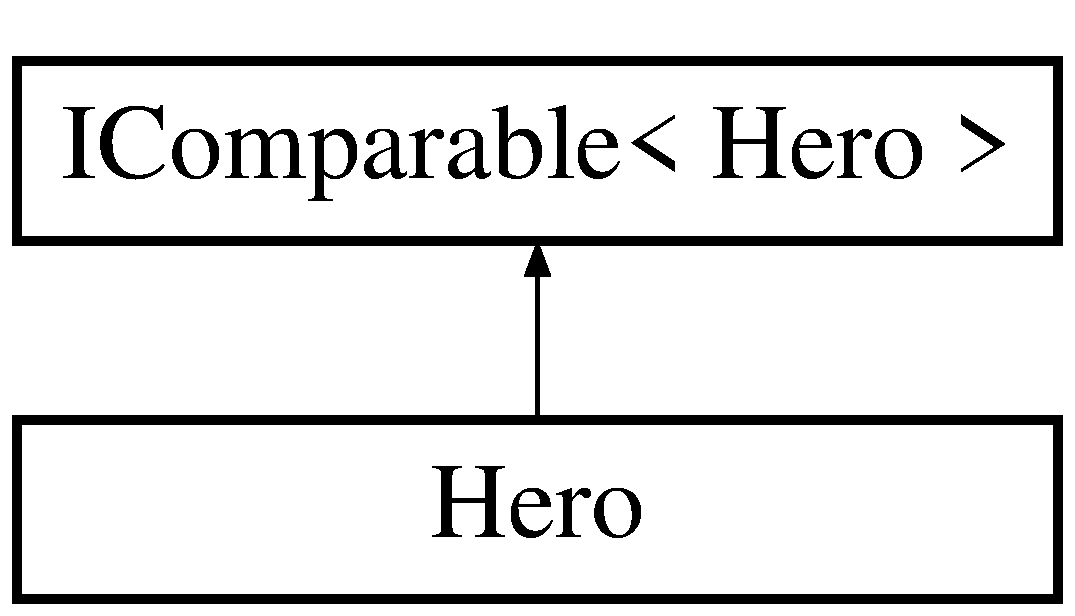
\includegraphics[height=2.000000cm]{class_hero}
\end{center}
\end{figure}
\subsection*{Открытые члены}
\begin{DoxyCompactItemize}
\item 
\mbox{\Hypertarget{class_hero_a85263cec7e8aabec935235b654a8dc1d}\label{class_hero_a85263cec7e8aabec935235b654a8dc1d}} 
{\bfseries Hero} (string name, int level)
\item 
\mbox{\Hypertarget{class_hero_a970d338ead03e94305770e039a0d1044}\label{class_hero_a970d338ead03e94305770e039a0d1044}} 
int {\bfseries Compare\+To} (\mbox{\hyperlink{class_hero}{Hero}} other)
\item 
\mbox{\Hypertarget{class_hero_add924381f82f8c5fd9c6abf46b9fac8e}\label{class_hero_add924381f82f8c5fd9c6abf46b9fac8e}} 
void {\bfseries Attack} ()
\item 
\mbox{\Hypertarget{class_hero_a40c63a9f068f6fceca81edbcf243868f}\label{class_hero_a40c63a9f068f6fceca81edbcf243868f}} 
void {\bfseries Defend} ()
\item 
\mbox{\Hypertarget{class_hero_af173b221c0d4c5b0e6bac9783ab834e0}\label{class_hero_af173b221c0d4c5b0e6bac9783ab834e0}} 
void {\bfseries Level\+Up} ()
\item 
\mbox{\Hypertarget{class_hero_a8474afa1cc7f3fc161af8c5aff8570d6}\label{class_hero_a8474afa1cc7f3fc161af8c5aff8570d6}} 
void {\bfseries Gain\+Experience} (int experience)
\item 
\mbox{\Hypertarget{class_hero_ab1f5d953931fd2e30ad54a97bb53a694}\label{class_hero_ab1f5d953931fd2e30ad54a97bb53a694}} 
void {\bfseries Display\+Info} ()
\end{DoxyCompactItemize}
\subsection*{Свойства}
\begin{DoxyCompactItemize}
\item 
\mbox{\Hypertarget{class_hero_a62211b255b5024a0002e2d3c967b2eb5}\label{class_hero_a62211b255b5024a0002e2d3c967b2eb5}} 
string {\bfseries Name}\hspace{0.3cm}{\ttfamily  \mbox{[}get, set\mbox{]}}
\item 
\mbox{\Hypertarget{class_hero_afd3f7dbef02fc8377d505d331bac884d}\label{class_hero_afd3f7dbef02fc8377d505d331bac884d}} 
int {\bfseries Level}\hspace{0.3cm}{\ttfamily  \mbox{[}get, set\mbox{]}}
\end{DoxyCompactItemize}


Объявления и описания членов класса находятся в файле\+:\begin{DoxyCompactItemize}
\item 
Program.\+cs\end{DoxyCompactItemize}

\hypertarget{class_program}{}\section{Класс Program}
\label{class_program}\index{Program@{Program}}


Объявления и описания членов класса находятся в файле\+:\begin{DoxyCompactItemize}
\item 
Program.\+cs\end{DoxyCompactItemize}

%--- End generated contents ---

% Index
\backmatter
\newpage
\phantomsection
\clearemptydoublepage
\addcontentsline{toc}{chapter}{Алфавитный указатель}
\printindex

\end{document}
